\section{L'azienda}
VisioneImpresa è un'azienda con quarant'anni di esperienza nell'offrire a piccole e medie imprese soluzioni informatiche per la 
gestione e l'automazione dei processi aziendali. I suoi prodotti di punta sono infatti sistemi ERP (\textit{Enterprise 
Resource Planning}) ovvero sistemi che permettono di coordinare il flusso di dati tra i processi di un'azienda, fornendo un'unica fonte di 
informazioni e semplificandone le operazioni.\\
VisioneImpresa è situata a Pernumia (Padova) e opera in prevalenza nel Nord Est, dal 2016 è entrata a far parte del gruppo Officegroup, azienda 
che riunisce diverse \textit{software house} specializzate nella progettazione e sviluppo di sistemi gestionali evoluti.\\
Dal 2023 inoltre VisioneImpresa è diventata una società benefit, ovvero è un azienda che opera con l'obiettivo di generare un impatto positivo 
sulla società e sull'ambiente, oltre al profitto finanziario.
Questo si realizza in diverse con iniziative che portano ad investire nelle energie rinnovabili e la sostenibilità, come 
l'incoraggiamento da parte dell'azienda ad usare bottiglie in vetro per l'acqua che vengono periodicamente ritirate e 
riutilizzate, o l'investimento in tecnologie ad alta efficienza energetica.\\
Altri obbiettivi perseguiti da questo tipo di attività sono la dematerializzazione e digitalizzazione, rispetto della parità di 
genere, formazione professionale del lavoratore, politiche a sostegno della conciliazione vita-lavoro, progetti con scuole ed 
università, co-progettazione con associazioni e istituzioni del territorio in ambito CSR 
(\textit{Corporate Social Responsability}) con il duplice obiettivo di stimolare la partecipazione dei dipendenti a 
“buone cause” della comunità e valorizzare il lavoro di associazioni no-profit del territorio, generando così valore sociale.

\begin{figure}[H]
    \centering
    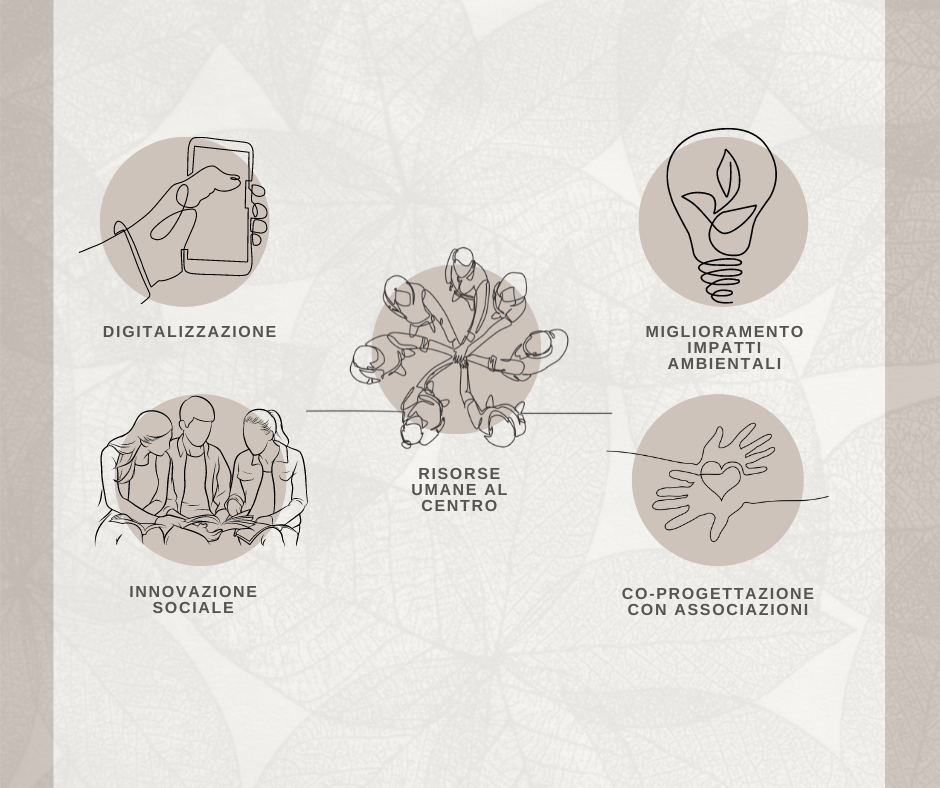
\includegraphics[alt={Obbiettivi delle società benefit}, width=0.5\textwidth]{img/soc-benefit.png}
    \caption{Obbiettivi delle società benefit}
    \label{fig:società benefit}
\end{figure}